\chapter{Another 16\textsuperscript{4} Tunes} 
\label{sec:torusmusic}

It's possible to dig into the making of the title music and how Jeff Minter
arrived at the music configuration he did thanks to a number of tiny demo programs that
survive from the period when he was developing Iridis Alpha.

Jeff distributed these little toys on `Compunet` in the summer of 1986. `Compunet' was a
predecessor to the modern internet that enabled C64 users with the equipment and
determination to dial up a local computer server over telephone landlines. Once dialled in,
they could participate in message boards and exchange and download files such as the little
\icode{prg} demos that Jeff Minter created here, 
\href{https://github.com/mwenge/iridisalpha/tree/master/demos/torus}{\textcolor{blue}{\icode{torus.prg}}}
and
\href{https://github.com/mwenge/iridisalpha/tree/master/demos/torus2}{\textcolor{blue}{\icode{torus2.prg}}}.

It turns out that Minter was heavily inspired by an article in 'Byte' magazine from June 1986.
This article, 'Musical Fractals' by Charles Dodge and Curtis Bahn  outlined a version of the
algorithm that Jeff ultimately adopted. The 'self-similarity' we encountered
in the way the Iridis Alpha theme tunes are constructed, a four-note structure\index{structure}
repeated across different time intervals on each of the three voices, finds its
roots in this article. The basic concept of layering we encountered in the previous chapter is illustrated using a tree diagram. The musical phrase played
at the top-most level is spread out in time in the levels above:

\begin{figure}[H]
  {
    \begin{adjustbox}{width=9cm,center}
      \frame{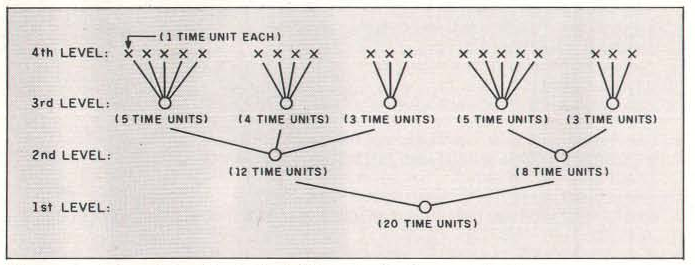
\includegraphics[width=11cm]{torus/fractal_illustration.png}}%
    \end{adjustbox}
  }\caption[]{The layering of the same notes across different time intervals, from \href{https://archive.org/details/byte-magazine-1986-06/page/n191/mode/2up}{\textcolor{blue}{'Musical Fractals'}}}
\end{figure}

The listings given in the article were in \icode{BASIC} and inscrutable to anything but the most minute attention:
\begin{lstlisting}[escapechar=\%,caption=A snippet from \icode{VARIATN.BAS}\, a progam for determinate fractal and Brownian variation.]
200 REM FRACTAL ROUTINE 
205 PRINT"COMPUTING FRACTAL" 
210 FOR Am1 TO PN 
220 AP(A)=P(A)+RC:AD(A)=D(A) 
230 FOR 131 TO PN 
240 BC=BC+1: IF R -1 THEN GOSUB 700 
245 BP(BC).AP(A)+P(B)+RC:BD(BC).D(B)*D(A) 
250 FOR 0.1 TO PN 
260 CC.CC+1:IF R.1 THEN GOSUB 700 
270 CP(CC).1111,(BC)+P(C)+RC:CD(CC).D(C)*BEI(BC):DT.DT+GD(CG) 
280 NEXT C: NEXT B: NEXT A 
\end{lstlisting}


Certainly, Minter must have experimented with them in order to arrive at his own version of fractal music. But it seems much more likely
that what caught his eye were patterns such as this one, which in a way make the general idea obvious and intuitive to the casual
reader:
\begin{figure}[H]
  {
    \begin{adjustbox}{width=12cm,center}
      \frame{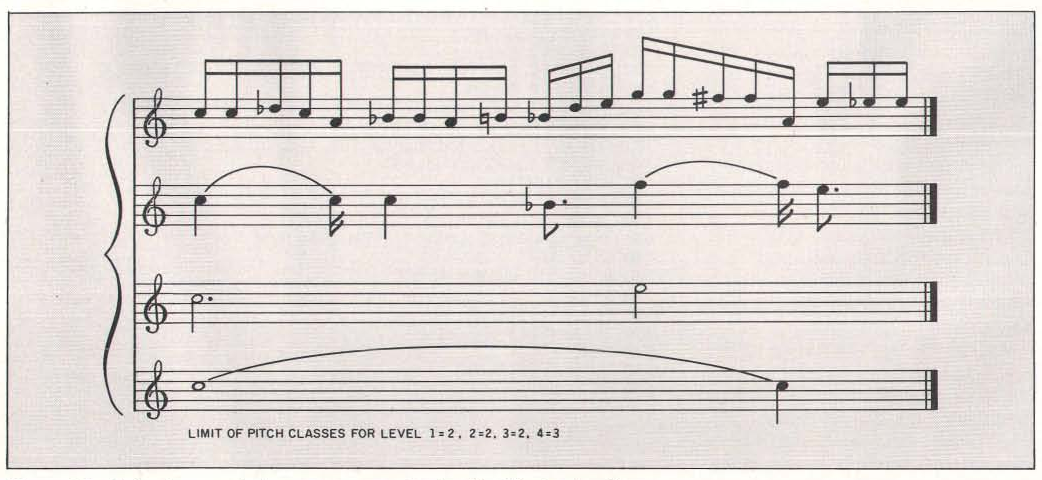
\includegraphics[width=11cm]{torus/fractal_notes.png}}%
    \end{adjustbox}
  }\caption[]{A pattern that looks familiar from our notation of Iridis Alpha's title music, from \href{https://archive.org/details/byte-magazine-1986-06/page/n191/mode/2up}{\textcolor{blue}{'Musical Fractals'}}}
\end{figure}

\section{Taurus:Torus}
\begin{figure}[H]
{
  \begin{adjustbox}{width=11cm,center}
  \includegraphics[width=11cm]{torus/torus.png}%
    \end{adjustbox}
}\caption[]{The splash screen for the Taurus:Torus demo.}
\end{figure}

This first demo, released in July 1986, has a version of Iridis' music-generating
algorithm that is nearly fully formed. However, the music it produces is quite
different. In fact, it is nearer to a tool for listening to and selecting music than
anything else.

The four seed values in \icode{titleMusicNoteArray\index{titleMusicNoteArray}} that are used to seed all subsequently
generated tunes (\icode{00 07 0C 07} in Iridis Alpha) can be selected and changed by the
user. They're called 'Oscillators' and each can be any value between 0 and 16, i.e. any of
\icode{0 1 2 3 4 5 6 7 8 9 A B C D E F}.

If we compare the title screen music routine from Iridis Alpha and the routine we find in \icode{Taurus:Torus} we can see that we
have a fractal-like self-similarity between the two going on. There are in fact only two points of difference, see if you can
spot them by glancing through the listings side by side:
\lstset{style=6502Style}
\lstinputlisting[caption=The music routine\index{routine} in Torus:Taurus side-by-side with Iridis Alpha.,basicstyle=\tiny\ttfamily]{torus/sidebyside.asm}

The Iridis Alpha routine has an extra step. At the very start it has a trapdoor for bailing out. This allows it control the duration
of the notes selected for playing:

\begin{lstlisting}[]
PlayTitleScreenMusic
        DEC baseNoteDuration
        BEQ MaybeStartNewTune
        RTS

MaybeStartNewTune   
        LDA previousBaseNoteDuration
        STA baseNoteDuration
\end{lstlisting}

The second difference lies in the placement of \icode{JSR SelectNewNotesToPlay}. The Torus demo selects new procedurally generated notes at every visit,
whereas the Iridis Alpha version only selects new notes at the beginning of a new 16 bar structure.
\begin{lstlisting}[]
       ; We'll only select a new tune when
       ; we've reached the beginning of a
       ; new 16 bar structure.            
       INX
       TXA
       AND #$03
       STA notesPlayedSinceLastKeyChange
       BNE MaybePlayVoice1

       JSR SelectNewNotesToPlay
\end{lstlisting}

When it runs, the demo cycles through procedural\index{procedural} configurations of \icode{titleMusicNoteArray\index{titleMusicNoteArray}} of 64 notes each.
In other words, exactly the kind of fractal structure\index{structure} we observed in Iridis Alpha proper. The examples below
give a flavour of the music it generates:

\begin{figure}[H]
{
  \begin{adjustbox}{width=14cm,center}
    \includegraphics[width=14cm]{torus/title_no_1_page_1001.png}}%
  \end{adjustbox}
}\caption[]{A pattern familiar from our discussion of the main title's music.}
\end{figure}

As before, the key to understanding the principle in operation here is that the four notes played by the entirety of 'Voice 1' are played in the first
four bars of 'Voice 2', and the first single bar of 'Voice 3'. The notes from each voice seed the notes selected for the other voices. Just as in our
discussion of the title tunes, the initial parameters chosen have a chaotic effect on the notes that are eventually played resulting in radically different
tunes from just small adjustments in initial values.

\begin{figure}[H]
{
  \begin{adjustbox}{width=14cm,center}
    \includegraphics[width=14cm]{torus/title_no_4_page_1001.png}}%
  \end{adjustbox}
}\caption[]{Tune 4 from Taurus:Torus}
\end{figure}


\clearpage
\section{A Graphical Interlude: Oscillator in 4 Parts}
Before we move on from Torus:Taurus, let's take a brief graphical diversion.
This demo was also  the laboratory where the elegant animation\index{animation} used when awarding a bonus was developed. 
\begin{figure}[H]
{
  \setlength{\tabcolsep}{3.0pt}
  \setlength\cmidrulewidth{\heavyrulewidth} % Make cmidrule = 
    \begin{adjustbox}{width=12cm,center}
  \begin{subfigure}{0.3\textwidth}
  \includegraphics[width=4cm]{torus/bonusbounty.png}%
  \end{subfigure}
  \begin{subfigure}{0.3\textwidth}
  \includegraphics[width=4cm]{torus/torus.png}%
  \end{subfigure}
  \end{adjustbox}
}\caption[]{The Torus oscillator animation\index{animation} and Iridis' bonus animation\index{animation}.}
\end{figure}

\begin{figure}[H]
  {
    \setlength{\tabcolsep}{3.0pt}
    \setlength\cmidrulewidth{\heavyrulewidth} % Make cmidrule = 
	\centering
	\def\MULTICOLORONE{red}
	\def\MULTICOLORTWO{white}
	\def\SPRITECOLOR{blue}
	\begin{subfigure}{0.5\textwidth}
		\input{sprites/LAND_GILBY1}
	\end{subfigure}
	\def\MULTICOLORONE{yellow}
	\def\MULTICOLORTWO{red}
	\def\SPRITECOLOR{c64_purple}
	\begin{subfigure}{0.5\textwidth}
		\input{sprites/BULLHEAD}
	\end{subfigure}
}\caption[position=top]{The sprites used in the Iridis Alpha bonus phase and the Torus demo.}
\end{figure}

The code handling each is identical and was only very lightly modified for the final game.
Starting with a side by side comparison of the two main routines we can see that the demo
code survived pretty much intact in Iridis Alpha.


\begin{minipage}[b]{0.45\linewidth}
\centering
\begin{lstlisting}[caption=Animation in Torus Demo,basicstyle=\tiny\ttfamily]
RunMainInterruptHandler   
        LDY #$00
        LDA #$F0
        STA $D012    ;Raster Pos
        DEC counterBetweeXPosUpdates
        BNE MaybeUpdateYPos

UpdateXPos
        LDA initialCounterBetweenXPosUpdates
        STA counterBetweeXPosUpdates

        LDA incrementForXPos
        CLC 
        ADC indexForXPosInSpritePosArray
        STA indexForXPosInSpritePosArray

MaybeUpdateYPos   
        DEC counterBetweenYPosUpdates
        BNE MaybeUpdateXPosOffset

        LDA initialCounterBetweenYPosUpdates
        STA counterBetweenYPosUpdates

        LDA indexForYPosInSpritePosArray
        CLC 
        ADC incrementForYPos
        STA indexForYPosInSpritePosArray

MaybeUpdateXPosOffset
        DEC cyclesBetweenXPosOffsetUpdates
        BNE MaybeUpdateYPosOffset

        LDA oscillator3Value
        STA cyclesBetweenXPosOffsetUpdates
        INC indexForXPosOffetsetInSpritePosArray

MaybeUpdateYPosOffset
        DEC cyclesBetweenYPosOffsetUpdates
        BNE StoreInitialIndexValues

        LDA oscillator4Value
        STA cyclesBetweenYPosOffsetUpdates
        INC indexForYPosOffsetInSpritePosArray

StoreInitialIndexValues   
        ; Store the initial values for our indices
        ; on the stack.
        LDA indexForXPosInSpritePosArray
        PHA 
        LDA indexForYPosInSpritePosArray
        PHA 
        LDA indexForXPosOffetsetInSpritePosArray
        PHA 
        LDA indexForYPosOffsetInSpritePosArray
        PHA 
\end{lstlisting}
\end{minipage}
\hspace{0.5cm}
\begin{minipage}[b]{0.45\linewidth}
\centering
\begin{lstlisting}[basicstyle=\tiny\ttfamily,caption=... and Iridis Alpha.,escapechar=\%]
AnimateGilbiesForNewBonus%\index{AnimateGilbiesForNewBonus}%
        LDY #$00
        LDA #$F0
        STA $D012    ;Raster Position
        DEC counterBetweeXPosUpdates%\index{counterBetweeXPosUpdates}%
        BNE MaybeUpdateYPos%\index{MaybeUpdateYPos}%

UpdateXPos
        LDA initialCounterBetweenXPosUpdates%\index{initialCounterBetweenXPosUpdates}%
        STA counterBetweeXPosUpdates%\index{counterBetweeXPosUpdates}%

        LDA incrementForXPos%\index{incrementForXPos}%
        CLC
        ADC indexForXPosInSpritePosArray%\index{indexForXPosInSpritePosArray}%
        STA indexForXPosInSpritePosArray%\index{indexForXPosInSpritePosArray}%

MaybeUpdateYPos%\index{MaybeUpdateYPos}%   
        DEC counterBetweenYPosUpdates%\index{counterBetweenYPosUpdates}%
        BNE MaybeResetOsc3WorkingValue%\index{MaybeResetOsc3WorkingValue}%

        LDA initialCounterBetweenYPosUpdates%\index{initialCounterBetweenYPosUpdates}%
        STA counterBetweenYPosUpdates%\index{counterBetweenYPosUpdates}%

        LDA indexForYPosInSpritePosArray%\index{indexForYPosInSpritePosArray}%
        CLC
        ADC incrementForYPos%\index{incrementForYPos}%
        STA indexForYPosInSpritePosArray%\index{indexForYPosInSpritePosArray}%

MaybeResetOsc3WorkingValue%\index{MaybeResetOsc3WorkingValue}%   
        DEC oscillator3WorkingValue%\index{oscillator3WorkingValue}%
        BNE MaybeResetOsc4WorkingValue%\index{MaybeResetOsc4WorkingValue}%

        LDA oscillator3Value%\index{oscillator3Value}%
        STA oscillator3WorkingValue%\index{oscillator3WorkingValue}%
        INC indexForXPosOffetsetInSpritePosArray%\index{indexForXPosOffetsetInSpritePosArray}%

MaybeResetOsc4WorkingValue%\index{MaybeResetOsc4WorkingValue}%   
        DEC oscillator4WorkingValue%\index{oscillator4WorkingValue}%
        BNE InitializeSpriteAnimation%\index{InitializeSpriteAnimation}%

        LDA oscillator4Value%\index{oscillator4Value}%
        STA oscillator4WorkingValue%\index{oscillator4WorkingValue}%
        INC inxedForYPosOffsetInSpritePosArray%\index{inxedForYPosOffsetInSpritePosArray}%

InitializeSpriteAnimation%\index{InitializeSpriteAnimation}%   
        ; Store the initial values for our indices
        ; on the stack.
        LDA indexForXPosInSpritePosArray%\index{indexForXPosInSpritePosArray}%
        PHA
        LDA indexForYPosInSpritePosArray%\index{indexForYPosInSpritePosArray}%
        PHA
        LDA indexForXPosOffetsetInSpritePosArray%\index{indexForXPosOffetsetInSpritePosArray}%
        PHA
        LDA inxedForYPosOffsetInSpritePosArray%\index{inxedForYPosOffsetInSpritePosArray}%
        PHA
\end{lstlisting}
\end{minipage}

To start getting a handle on how the oscillation animation\index{animation} works, lets plot the first 24 animations that the Torus
demo uses when left to its own devices. We get a variety of different trajectories, some relatively simple, some
quite convoluted.

\clearpage
\begin{figure}[p]
    \centering
    \foreach \l in {0, ..., 23}
    {
      \begin{subfigure}{0.3\textwidth}
        \begin{tikzpicture}
        \begin{axis}[
          xmin = 0, xmax = 150,
               ymin = 0, ymax = 256,
               xtick distance = 50,
               ytick distance = 50,
               grid = both,
               minor tick num = 10,
               major grid style = {lightgray},
               minor grid style = {lightgray!25},
               width = \textwidth,
               height = 0.75\textwidth,
               legend cell align = {left},
               legend pos = north west,
               font = \tiny\ttfamily
        ]
        \addplot[blue, ultra thin, mark = *,mark size=0.4pt] table [x = {x}, y = {y}] {src/torus/Oscillation\l.dat};
        \end{axis}
        \end{tikzpicture}
      \end{subfigure}
    }%
\caption{The first 24 oscillation patterns generated by the Torus demo.}
\end{figure}
\clearpage

When we look into the code we find this petting zoo of animations is principally driven by a simple sequence\index{sequence}
of bytes stored in \icode{spritePositionArray}.

\CopyPartialFile{../iridisalpha/demos/torus/src/torus.asm}{tmp.asm}{243}{251}%
\lstinputlisting[]{tmp.asm}

We can get a sense of how this rising and falling sequence\index{sequence} of values can be used to plot a course across the screen\index{screen}
if we treat each as an x and y value on a graph of cartesian co-ordinates. In the twenty four instances below we
start by treating the value as providing both the x and y position. In each subsequent one we skip an increasing
number of positions ahead in the sequence\index{sequence} to get the y value, producing a variety of elliptical orbits around
the screen\index{screen}. 

\begin{figure}[H]
    \centering
    \foreach \l in {0, ..., 11}
    {
      \begin{subfigure}{0.3\textwidth}
        \begin{tikzpicture}
        \begin{axis}[
          xmin = 0, xmax = 256,
               ymin = 0, ymax = 256,
               xtick distance = 50,
               ytick distance = 50,
               grid = both,
               minor tick num = 10,
               major grid style = {lightgray},
               minor grid style = {lightgray!25},
               width = \textwidth,
               height = 0.75\textwidth,
               legend cell align = {left},
               legend pos = north west,
               font = \tiny\ttfamily
        ]
        \addplot[blue, ultra thin, mark = *,mark size=0.4pt] table [x = {x}, y = {y}] {src/torus/OscillationRaw-\l.dat};
        \end{axis}
        \end{tikzpicture}
      \end{subfigure}
    }%
\caption{Using the x/y offset in \icode{spritePositionArray} where y is the value after x in the array.}
\end{figure}

To get beyond simple ellipsoids we need to do more than pick a different value in the array for our x and y offsets.
Here we experiment with something a little more involved. We update the x and y positions at different intervals
and when skipping ahead in \icode{spritePositionArray} for a new value for x and y we use a pre-selected, random
number of bytes to skip past.

\begin{figure}[H]
    \centering
    \foreach \l in {0, ..., 11}
    {
      \begin{subfigure}{0.3\textwidth}
      \includegraphics[width=4cm]{torus/OscillationTest\l.png}%
      \end{subfigure}
    }%
\caption{Testing different values of x and y}
\end{figure}

This is starting to look more like the actual results we observed and it is where the 4 values selectable by the player using keys z, x, c, and v in the Torus demo come in. In addition
to controlling the music generation procedure, as we've already seen, they also determine the way the values in
\icode{spritePositionArray} are selected for position the sprite in each new frame. This is based on letting them
determine the frequency\index{frequency} with which the position of the x and y values of each sprite is changed and how far to skip
ahead in \icode{spritePositionArray} when selecting a new value from it for the x and y position.


\begin{figure}[H]
  {
    \setlength{\tabcolsep}{3.0pt}
    \setlength\cmidrulewidth{\heavyrulewidth} % Make cmidrule = 
    \begin{adjustbox}{width=12cm,center}

      \begin{tabular}{rllllllll}
        \toprule
        Key & Name & Purpose & Code &\\
        \midrule
Z & Oscillator 1 & \makecell[l]{
- Intervals between updating X position.\\
- The amount to increment the index into\\
\icode{spritePositionArray}\\
when getting the next X position.\\
} & \makecell[l]{
\CopyPartialFile{../iridisalpha/demos/torus/src/torus.asm}{tmp.asm}{735}{751}%
\lstinputlisting[linewidth=5cm,basicstyle=\tiny\ttfamily]{tmp.asm}
} \\
        \midrule
X & Oscillator 2 & \makecell[l]{
- Intervals between updating Y position.\\
- The amount to increment the index into \\
\icode{spritePositionArray}\\
when getting the next Y position.\\
} & \makecell[l]{
\CopyPartialFile{../iridisalpha/demos/torus/src/torus.asm}{tmp.asm}{753}{768}%
\lstinputlisting[linewidth=5cm,basicstyle=\tiny\ttfamily]{tmp.asm}
} \\
        \midrule
C & Oscillator 3 & \makecell[l]{
- How often to increase the index that seeks \\
ahead to get a value\\
from \icode{spritePositionArray}for adding \\
to the next X position.\\
} & \makecell[l]{
\CopyPartialFile{../iridisalpha/demos/torus/src/torus.asm}{tmp.asm}{770}{780}%
\lstinputlisting[linewidth=5cm,basicstyle=\tiny\ttfamily]{tmp.asm}
} \\
        \midrule
V & Oscillator 4 & \makecell[l]{
- How often to increase the index that seeks \\
ahead to get a value\\
from \icode{spritePositionArray}for adding \\
to the next Y position.\\
} & \makecell[l]{
\CopyPartialFile{../iridisalpha/demos/torus/src/torus.asm}{tmp.asm}{782}{791}%
\lstinputlisting[linewidth=5cm,basicstyle=\tiny\ttfamily]{tmp.asm}
} \\
        \addlinespace
        \bottomrule
      \end{tabular}
    \end{adjustbox}
  }\caption{The purpose of each of the oscillator values.}
\end{figure}

In \icode{RunMainInterruptHandler} we can see how each of these values
set by the player is used to maintain an accounting of the different sprite positions for each of the 8 sprites\index{sprites}:

\CopyPartialFile{../iridisalpha/demos/torus/src/torus.asm}{tmp.asm}{361}{403}%
\lstinputlisting[]{tmp.asm}

Before animating each of the 8 sprites\index{sprites} we use the values set by the player to prepare the variables
that will be applied to positioning each sprite. For example the value selected with the Z key has been
used to set \icode{initialCounterBetweenXPosUpdates\index{initialCounterBetweenXPosUpdates}} and \icode{incrementForXPos\index{incrementForXPos}}. In the first lines above
in \icode{UpdateXPos} we use them to set up \icode{indexForXPosInSpritePositionArray\index{indexForXPosInSpritePositionArray}}. THis is then used
in \icode{SpriteAnimationLoop\index{SpriteAnimationLoop}} to selec the X position of the current sprite:


\CopyPartialFile{../iridisalpha/demos/torus/src/torus.asm}{tmp.asm}{419}{424}%
\lstinputlisting[]{tmp.asm}

You can follow the same lineage between the setting of each value in our table above with the rest of the
\icode{SpriteAnimationLoop\index{SpriteAnimationLoop}} routine\index{routine}.

\clearpage
\begin{definition}[A Testing Hack]
\setlength{\intextsep}{0pt}%
\setlength{\columnsep}{3pt}%
\small
It's not easy to create a bonus animation and test it unless you plan to play through the game each time until you earn a bonus. For that
  reason it makes sense to have some way of calling up the bonus routine quick-and-dirty-like.
  In the CheckKeyboardInGame\index{CheckKeyboardInGame} routine, we find the following:
\begin{lstlisting}[basicstyle=\tiny\ttfamily,escapechar=\%]
        ; We can award ourselves a bonus bounty by
        ; pressing Y at any time, as long as '1C' is the
        ; first character%\index{character}% in the hiscore table. Not sure
        ; what this hack is for, testing?
CheckYPressed%\index{CheckYPressed}%   
        CMP #KEY_Y ; Y Pressed
        BNE ReturnFromKeyboardCheck%\index{ReturnFromKeyboardCheck}%
        LDA canAwardBonus%\index{canAwardBonus}%
        CMP #$1C
        BNE ReturnFromKeyboardCheck%\index{ReturnFromKeyboardCheck}%
        INC bonusAwarded%\index{bonusAwarded}%
        RTS
\end{lstlisting}

In the above the `canAwardBonus\index{canAwardBonus}` byte is the first letter in the name of the player with the top score in the Hi-Score table. By default this is 'YAK':

\begin{lstlisting}[basicstyle=\tiny\ttfamily,escapechar=\%]
;-------------------------------------------------------
; The high score table.
;-------------------------------------------------------
hiScoreTablePtr%\index{hiScoreTablePtr}%           .TEXT "0068000"
canAwardBonus%\index{canAwardBonus}%             .TEXT "YAK "
                          .FILL 10, $00
                          .TEXT  "0065535RATT"
                          .FILL 10, $00
\end{lstlisting}
But if we change 'Y' to \icode{\$1C} like so, we can activate the hack:

\begin{lstlisting}[basicstyle=\tiny\ttfamily,escapechar=\%]
hiScoreTablePtr%\index{hiScoreTablePtr}%           .TEXT "0068000"
canAwardBonus%\index{canAwardBonus}%             .TEXT $1C,"AK "
\end{lstlisting}

Note that \icode{\$1C} is charset\index{charset} code for a bull's head symbol in Iridis Alpha, so it is also possible to enter this as the initial of a high scorer name if we get a score that puts us to the top of the table:

\CopyPartialFile{../iridisalpha/src/graphics/charset.asm}{tmp.asm}{287}{296}%
\lstinputlisting[basicstyle=\tiny\ttfamily]{tmp.asm}


I'm guessing this was used for testing the animation\index{animation} routine\index{routine} and left in as an Easter egg.
\end{definition}

\section{Taurus/Torus Two}
\begin{figure}[H]
{
  \begin{adjustbox}{width=11cm,center}
  \includegraphics[width=11cm]{torus/torus2.png}%
    \end{adjustbox}
}\caption[]{Now even freakier you say.}
\end{figure}

In this second iteration of the Taurus:Torus demo, the theme tune for the main game has crystallized. The routines are now sufficiently identical
that they produce the same output. The initial settings produced the Iridis Alpha theme tune as it was in the game's final release.

\lstset{style=6502Style}
\lstinputlisting[caption=The music routine\index{routine} in Taurus:Torus II side-by-side with Iridis Alpha.,basicstyle=\tiny\ttfamily]{torus/sidebyside2.asm}


\begin{figure}[H]
{
  \begin{adjustbox}{width=14cm,center}
    \includegraphics[width=14cm]{torus/torus2_title_no_1_page_1001.png}%
  \end{adjustbox}
}\caption[]{The music produced by Taurus/Torus Two. This is note for note identical to the theme tune in the final game below.}
\end{figure}

\begin{figure}[H]
{
  \begin{adjustbox}{width=14cm,center}
    \includegraphics[width=14cm]{music/title_no_1_page_1001.png}%
  \end{adjustbox}
}
\end{figure}

